\documentclass[10pt,fleqn]{article} % Default font size and left-justified equations
\usepackage{import}
\usepackage[%
    pdftitle={Energie et puissance d'un smartphone},
    pdfauthor={Geoffrey Vaquette}]{hyperref}
\subimport{../../../../style/}{preambule}
%\fichetrue
\fichefalse

%\proftrue
\proffalse

\tdtrue
%\tdfalse

\courstrue
%\coursfalse

\subimport{../../../../style/}{new_style}
\subimport{../../../../style/}{macros_SII}
\subimport{../../../../style/}{preambule_trou}

\usepackage{siunitx}
% -------------------------------------
% Déclaration des titres
% -------------------------------------

\def\discipline{Enseignement \\Technologique \\ Transversal}
\def\xxtete{Enseignement Technologique Transversal}

\def\classe{1 STI2D}
\def\xxnumpartie{Séquence 2}
\def\xxpartie{Energie électrique et puissance d'un smartphone}

\def\xxnumchapitre{Séance 3}
\def\xxchapitre{\hspace{.12cm} Énergies, Puissances et rendement}

\def\xxposongletx{2}
\def\xxposonglettext{1.45}
\def\xxposonglety{23}
\def\xxonglet{Seq. 2 -- DS 3}

\def\xxactivite{DS}
\def\xxauteur{\textsl{Geoffrey Vaquette}}

\def\xxcompetences{%
\textsl{%
\textbf{Savoirs et compétences :}
\begin{itemize}[label=\ding{112},font=\color{ocre}]
\item CO2.1	Identifier les flux et la forme de l'énergie, caractériser ses transformations et/ou modulations et estimer l'efficacité globale d'un système.
\end{itemize}
%
}}

\def\xxfigures{
\begin{center}
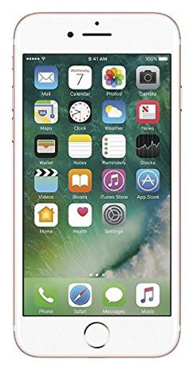
\includegraphics[height=4cm]{images/smartphone.png} \\
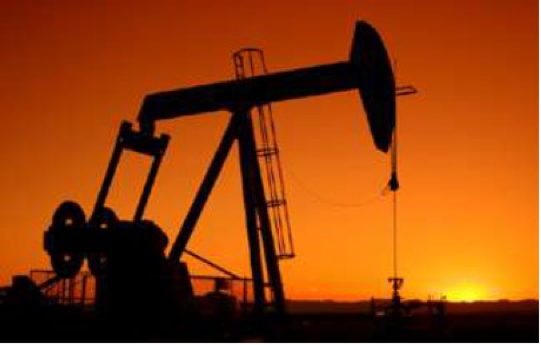
\includegraphics[height=4cm]{images/petrole.png} \\
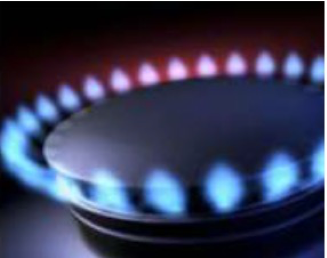
\includegraphics[height=4cm]{images/gaz.png} \\
\end{center}
}%figues de la page de garde
\def\xxpied{%
Energies, Puissances et Rendement \xxactivite%
}

%---------------------------------------------------------------------------

\renewcommand{\RemplirTrou}{true}
\begin{document}
\chapterimage{png/Fond_solaire}

\begin{obj}
Déterminer l’énergie et la puissance disponibles dans un système

L’étude suivante concerne un smartphone. 

Vous serez amené-e à
 calculer l’énergie présente dans la batterie de ce téléphone ainsi que les puissances et énergies nécessaires
 nécessaires pour différentes utilisations de celui-ci.
 
\end{obj}
\section{Introduction}
\begin{center}
    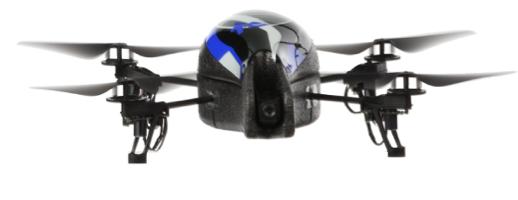
\includegraphics[height=0.1\textheight]{images/drone.png}
\end{center}
    

\subsection{Présentation du système}
L'AR.Drone de la société Parrot, a été le premier quadricoptère piloté par une tablette mobile connectée en Wi-Fi. L'AR.Drone n'est pas simplement un quadricoptère télécommande, c'est aussi le cœur d'une plate-forme de jeu a réalité augmentée multijoueur.
Il est conçu pour une utilisation en extérieur et en intérieur grâce a une carène prévue pour le protéger des chocs et pour éviter le contact avec les hélices en rotation.


% En plus du pilotage intuitif de l'AR.Drone par de simples mouvements appliqués au mobile, les cameras embarquées nous permettent d'avoir une vision en direct de l'aéronef sur l'écran du mobile a quelques dizaines de mètres grâce au réseau Wi-Fi établi entre l'AR.Drone et son mobile de pilotage. L'AR.Drone possède deux cameras, une frontale et l'autre verticale, pour donner une impression de perception en profondeur lors du vol et il est possible de sélectionner l'une ou l'autre des caméras (ou les deux) depuis l'application de pilotage.

L'AR.Drone dispose aussi de plusieurs fonctionnalités d'auto-pilotage permettant le décollage, l’atterrissage et le vol stationnaire. Le pilote automatique assure aussi le contrôle de l'AR.Drone en cas de perte de connexion Wi-Fi avec le mobile de pilotage. Si l'AR.Drone est utilisé avec un jeu a réalité augmentée, plusieurs fonctions de reconnaissance de formes permettent la détection de marqueurs placés au sol ou sur d'autres drones facilitant ainsi le guidage de l'aéronef.

\subsection{Diagramme de définition des blocs}

\begin{figure}[h!]
    \centering
    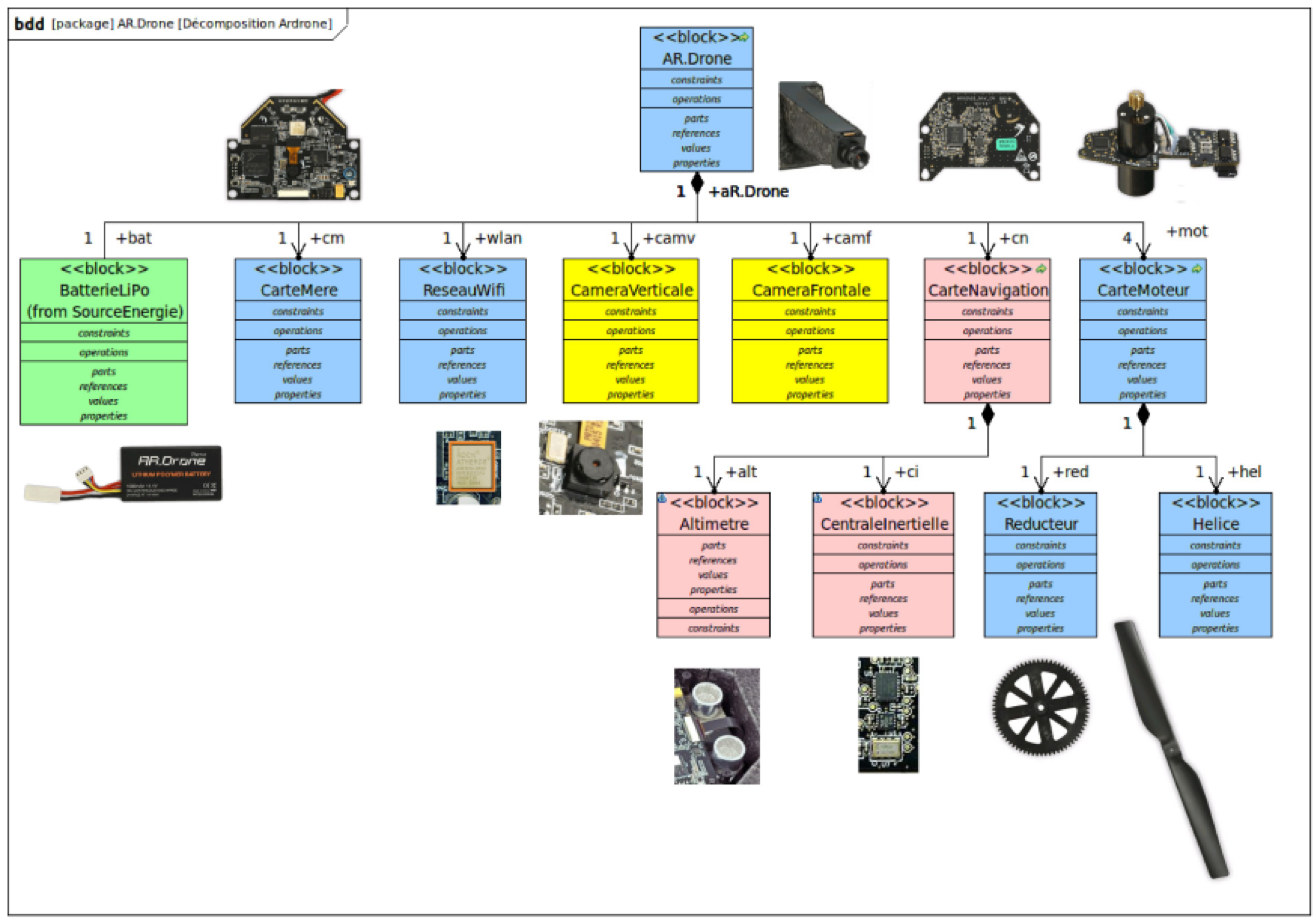
\includegraphics[width=0.9\textwidth]{images/bdd.png}
    \caption{Diagramme de définition des blocs simplifié}
    \label{fig:bdd}
\end{figure}



\section{Caractérisation de la chaîne d'énergie}
\begin{exercise}~

\begin{question}
  Citez deux types d'énergie qui interviennent dans ce système.
\end{question} 
\begin{solution}
  Les énergies intervenant dans ce système sont les énergies électriques et mécanique. 
\end{solution}

\begin{question}
    Quel(s) composant(s) permet(ent) de convertir l'énergie dans ce système ? D'après le diagramme de définition des blocs (Figure~\ref{fig:bdd}), combien le système en compte-t-il ? 
\end{question}
\begin{solution}
  Ce sont les moteurs (carte-moteur) qui permettent de convertir l'énergie électrique en énergie mécanique. On peut lire dans le bdd qu'il y a 4 cartes moteur. 
\end{solution}

\begin{question}
    A l'aide de la liste de composants ci-dessous, complétez la chaîne d'énergie. 
    \begin{itemize}
        \item Carte moteur
        \begin{itemize}
            \itemf Permet de contrôler la vitesse du moteur
        \end{itemize}
        \item Carte Wifi
        \item Engrenages
        \item Caméra
        \item Batterie Li-Ion
    \end{itemize}
    
    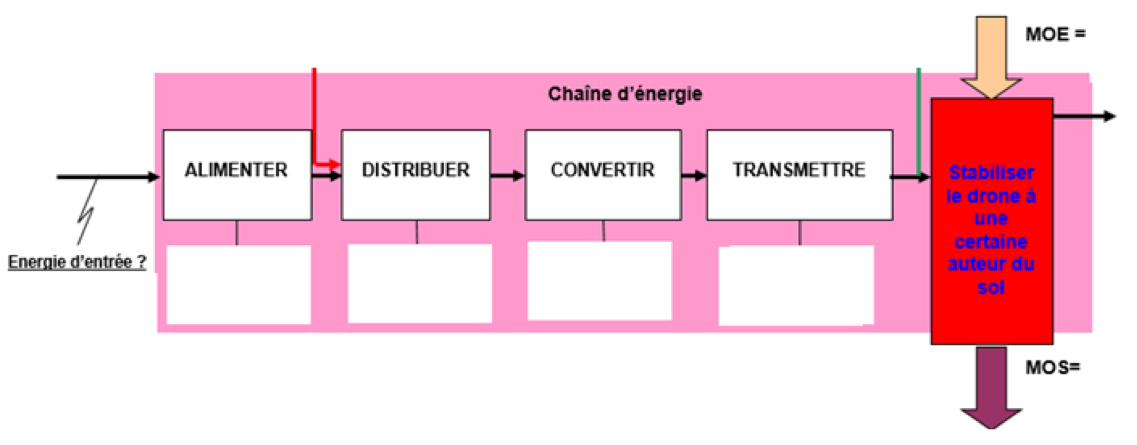
\includegraphics[width=\textwidth]{images/chaineenergie.png}
\end{question}
\end{exercise}
\pagebreak
\section{Etude énergétique du système}

\begin{figure}
    \centering
    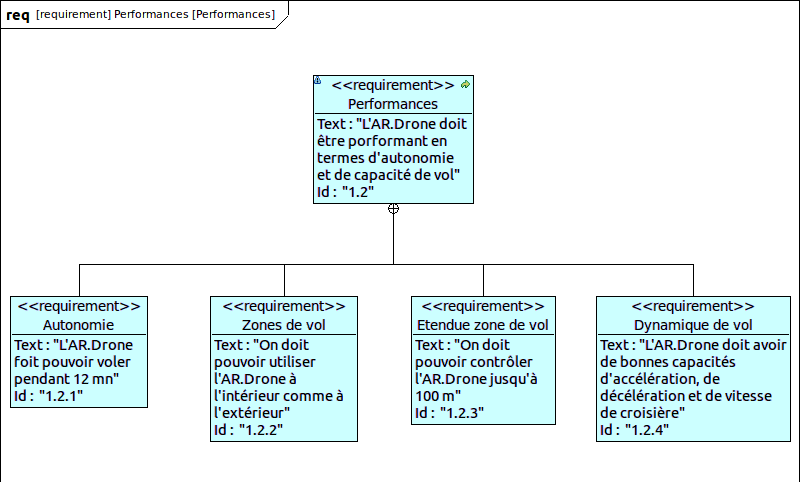
\includegraphics[height=0.3\textheight]{images/exigence_drone.png}
    \caption{Extrait du diagramme des exigences}
    \label{fig:exi}
\end{figure}

Le dossier technique donne les caractéristiques suivantes pour la \textbf{batterie} :
\begin{description}
 \item[Technologie :] Li-Pol (lithium-polymer)
\item[Capacité :] $ C = \SI{1000}{mAh} $
\item[Tension :] $U=\SI{11.1}{V}$
\item[Temps de charge :] \SI{90}{min}
\end{description}

Le dossier technique donne les caractéristiques principales suivantes pour un \textbf{moteur} : 
\begin{description}
    \item[Couple moyen en utilisation : ] $C = \SI{2.5e-3}{Nm}$
    \item[Tension moyenne en utilisation : ] $U = \SI{10}{V}$
    \item[Vitesse de rotation : ] $\Omega = \SI{40000}{tr/min}$
    \item[Rendement : ] $\alpha = 0.7$
\end{description}

Rappel de conversion : $$\SI{1}{tr/min} = \frac{2\pi}{60}\si{rad/s}$$

\begin{exercise}~

\begin{question}
  Calculer l’énergie électrique $E_\text{bat}$que contient la batterie. Donnez le résultat en Joules et en \si{Wh}
\end{question}
\begin{solution}
  On connaît la tension de la batterie, ainsi que sa capacité. L'énergie 
  contenue dans la batterie est $$\omega_\text{bat} = U\times C = 11.1 \times \num{1000e-3}=\SI{11.1}{Wh} $$
\end{solution}
\begin{question}
    Calculez la puissance $P_\text{meca}$ en utilisation consommée par chacun des moteurs.
    
    \textit{Rappel : En rotation, la puissance mécanique s'exprime $P = C\times \omega$ avec $C$ le couple déployé et $\omega$ la vitesse de rotation en $\si{rad/s}$.}
\end{question}
\begin{solution}
On connaît le couple développé et la vitesse de rotation en \si{tr/min}. On a $\omega = 40000\times \frac{2\pi}{60}$. $$P = C\times\omega = \num{2.5e-3}\times 40000 \times \frac{2\pi}{60} = \SI{10.5}{W} $$
\end{solution}

\begin{question}
  Connaissant le rendement du moteur, calculez la puissance électrique $P_\text{elec}$ consommée par un moteur. 
\end{question}
\begin{solution}
  On a $P_\text{meca} = \alpha P_\text{elec} \Rightarrow P_\text{elec} = \frac{P_\text{meca}}{\alpha} = \frac{10.5}{0.7} = \SI{15}{W}$
\end{solution}

\begin{question}
  Supposons à présent que le total des quatre moteurs consomme une puissance totale de $P_\text{tot} = \SI{60}{W}$.
  
  Calculez le courant total $I_\text{tot}$ alimentant les moteurs. 
\end{question}
\begin{solution}
  On a $P = U\times I \Rightarrow I = \frac{P}{U} = \frac{60}{10} = \SI{6}{A}$
\end{solution}

\begin{question}
    En considérant que seuls les moteurs consomme de l'électricité, calculez l'autonomie en vol. 
\end{question}


\begin{question}
    Le résultat précédent est-il satisfaisant vis-à-vis des exigences ? Justifiez.
\end{question}
\end{exercise}

\end{document}